%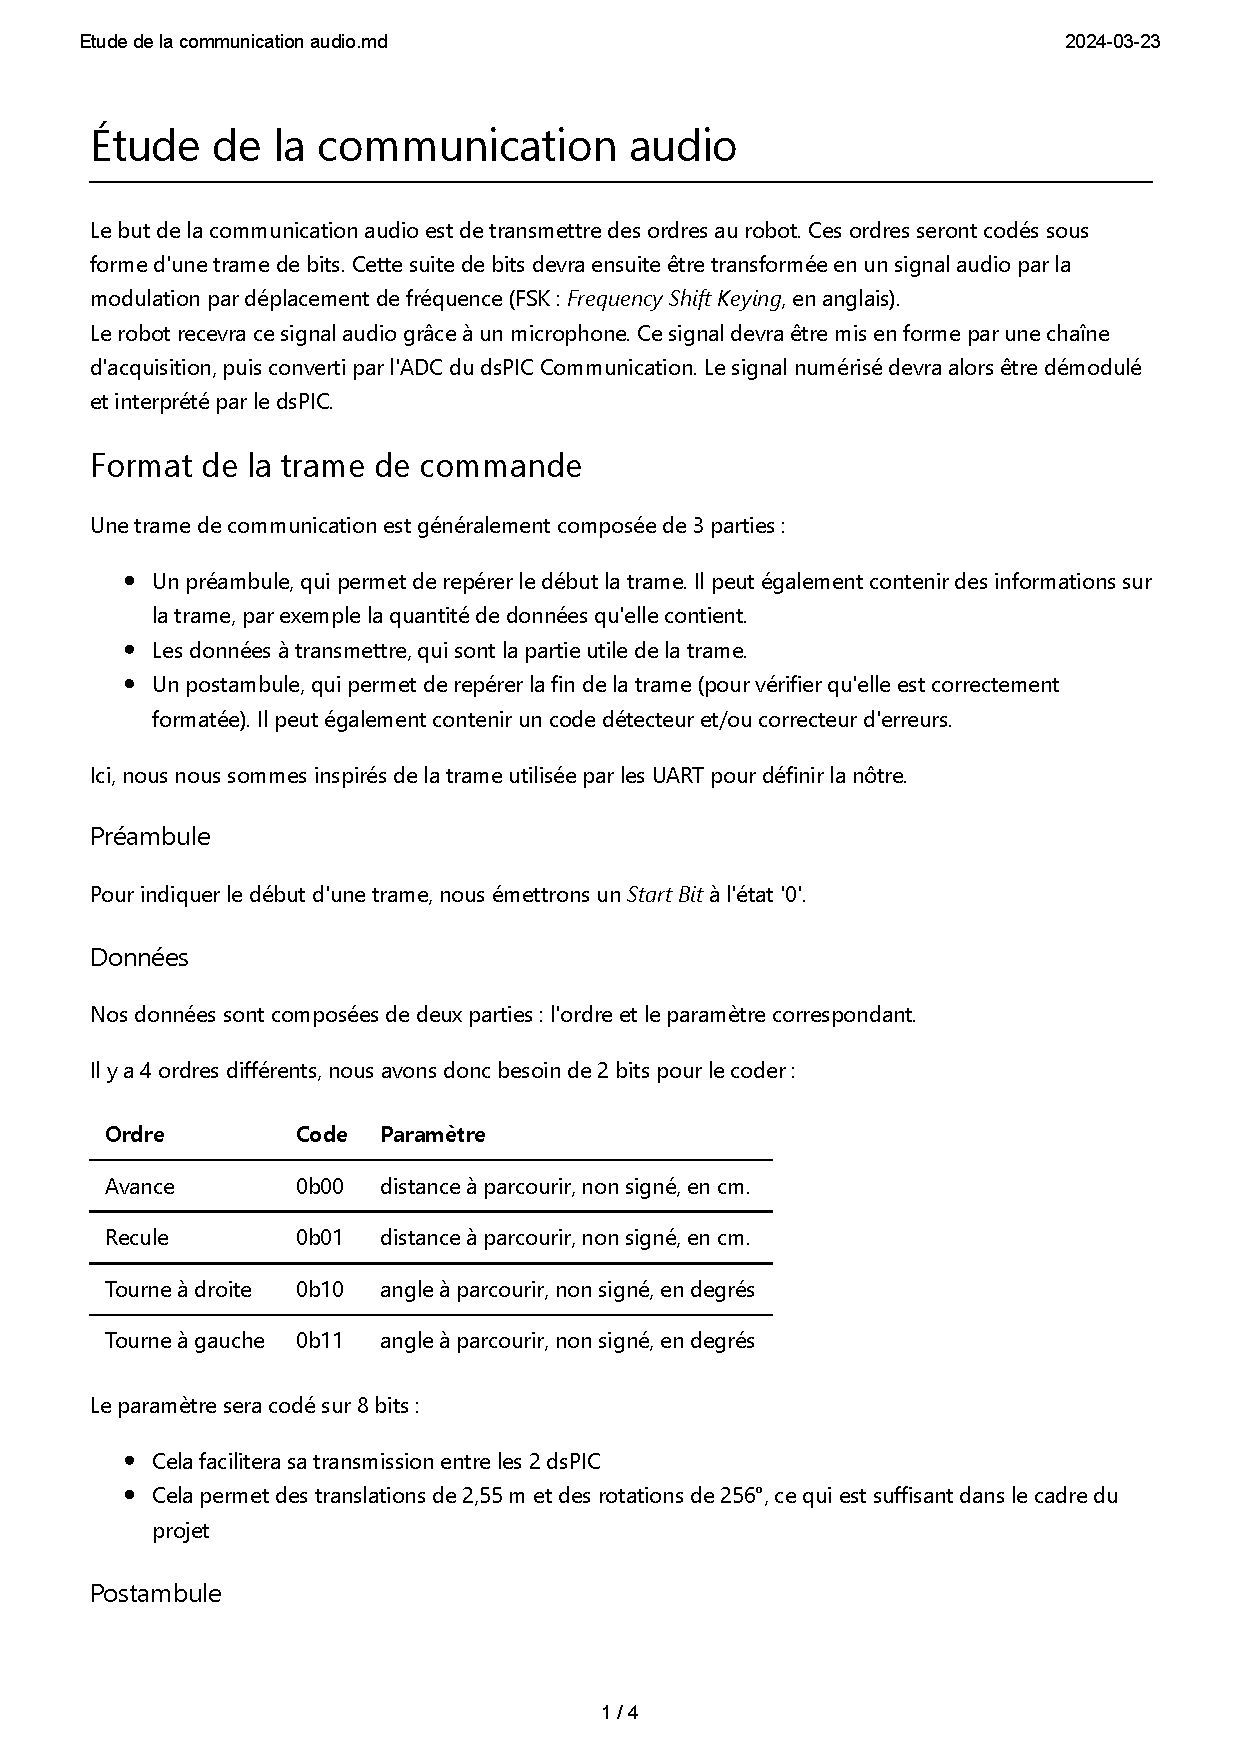
\includepdf[scale=0.8,pages=1,pagecommand={\section{Etude la communication audio}\label{etudecommmd}},linktodoc=true]{pdffiles/Etude de la communication audio.pdf} 
%\includepdf[scale=0.8,pages=2-]{pdffiles/Etude de la communication audio.pdf} 

\section{Filtre passe-haut} \label{hfilterannexe}
\begin{figure}[H]
    \centering
    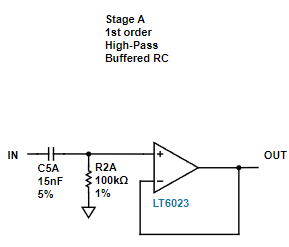
\includegraphics{Pictures/highpassfilter.png}
    \caption{Filtre passe-haut}
    \label{fig:highpassfilterannexe}
\end{figure}


\begin{figure}[H]
    \centering
    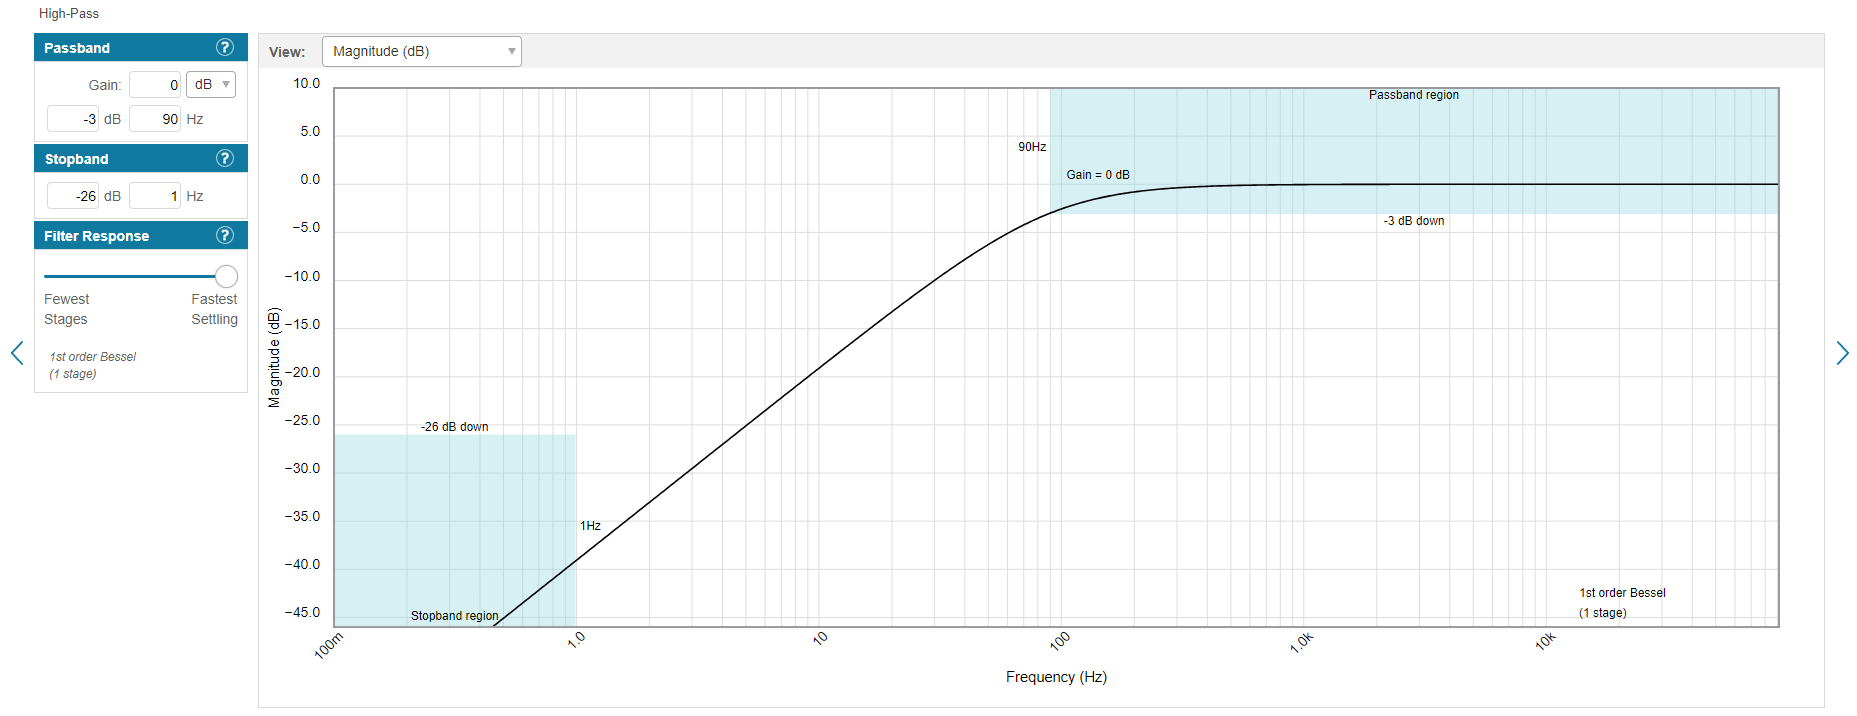
\includegraphics[width=1.5\textwidth,angle=90,origin=c]{Pictures/highpassspecs.png}
    \caption{Gain du filtre passe-haut en dB}
    \label{fig:highpassfiltermagnannexe}
\end{figure}

\newpage
\section{Simulation LTspice du filtre passe-haut avec polarisation} \label{ltspiceHighPassResistors}
\begin{figure}[H]
    \centering
    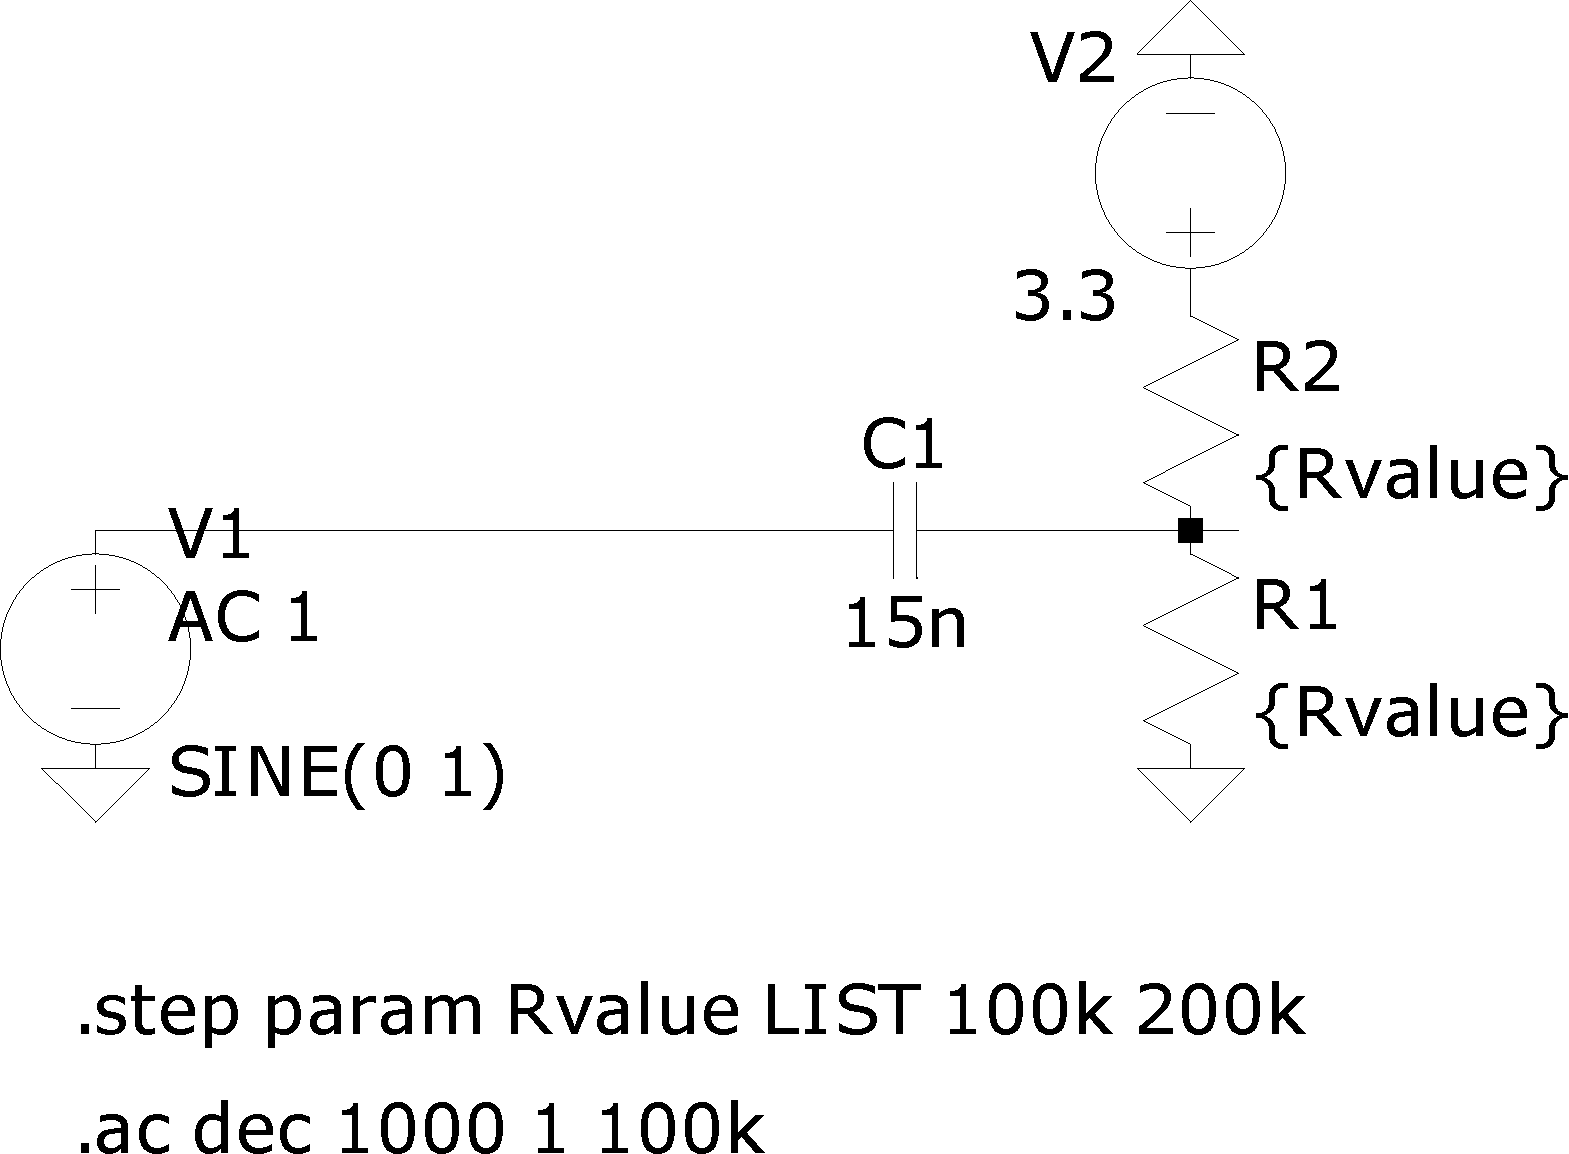
\includegraphics[width=0.7\textwidth]{pdffiles/HighPass/CircuitHighPassPolarization.pdf}
    \caption{Simulation LTspice du filtre passe-haut avec des résistances de polarisation variant de $100k$ à $200k$}
    \label{fig:ltspiceHighPassResistors}
\end{figure}


\includepdf[pages=3,pagecommand={\section{Datasheet MCP601}\label{datasheet}},linktodoc=true]{pdffiles/21314g.pdf}

\newpage
%\section{Comparaison réponse transitoire cas équivalent courant et transistor} \label{LTspiceCurrentvsJFTTransient}
%\begin{figure}[H]
%    \centering
%    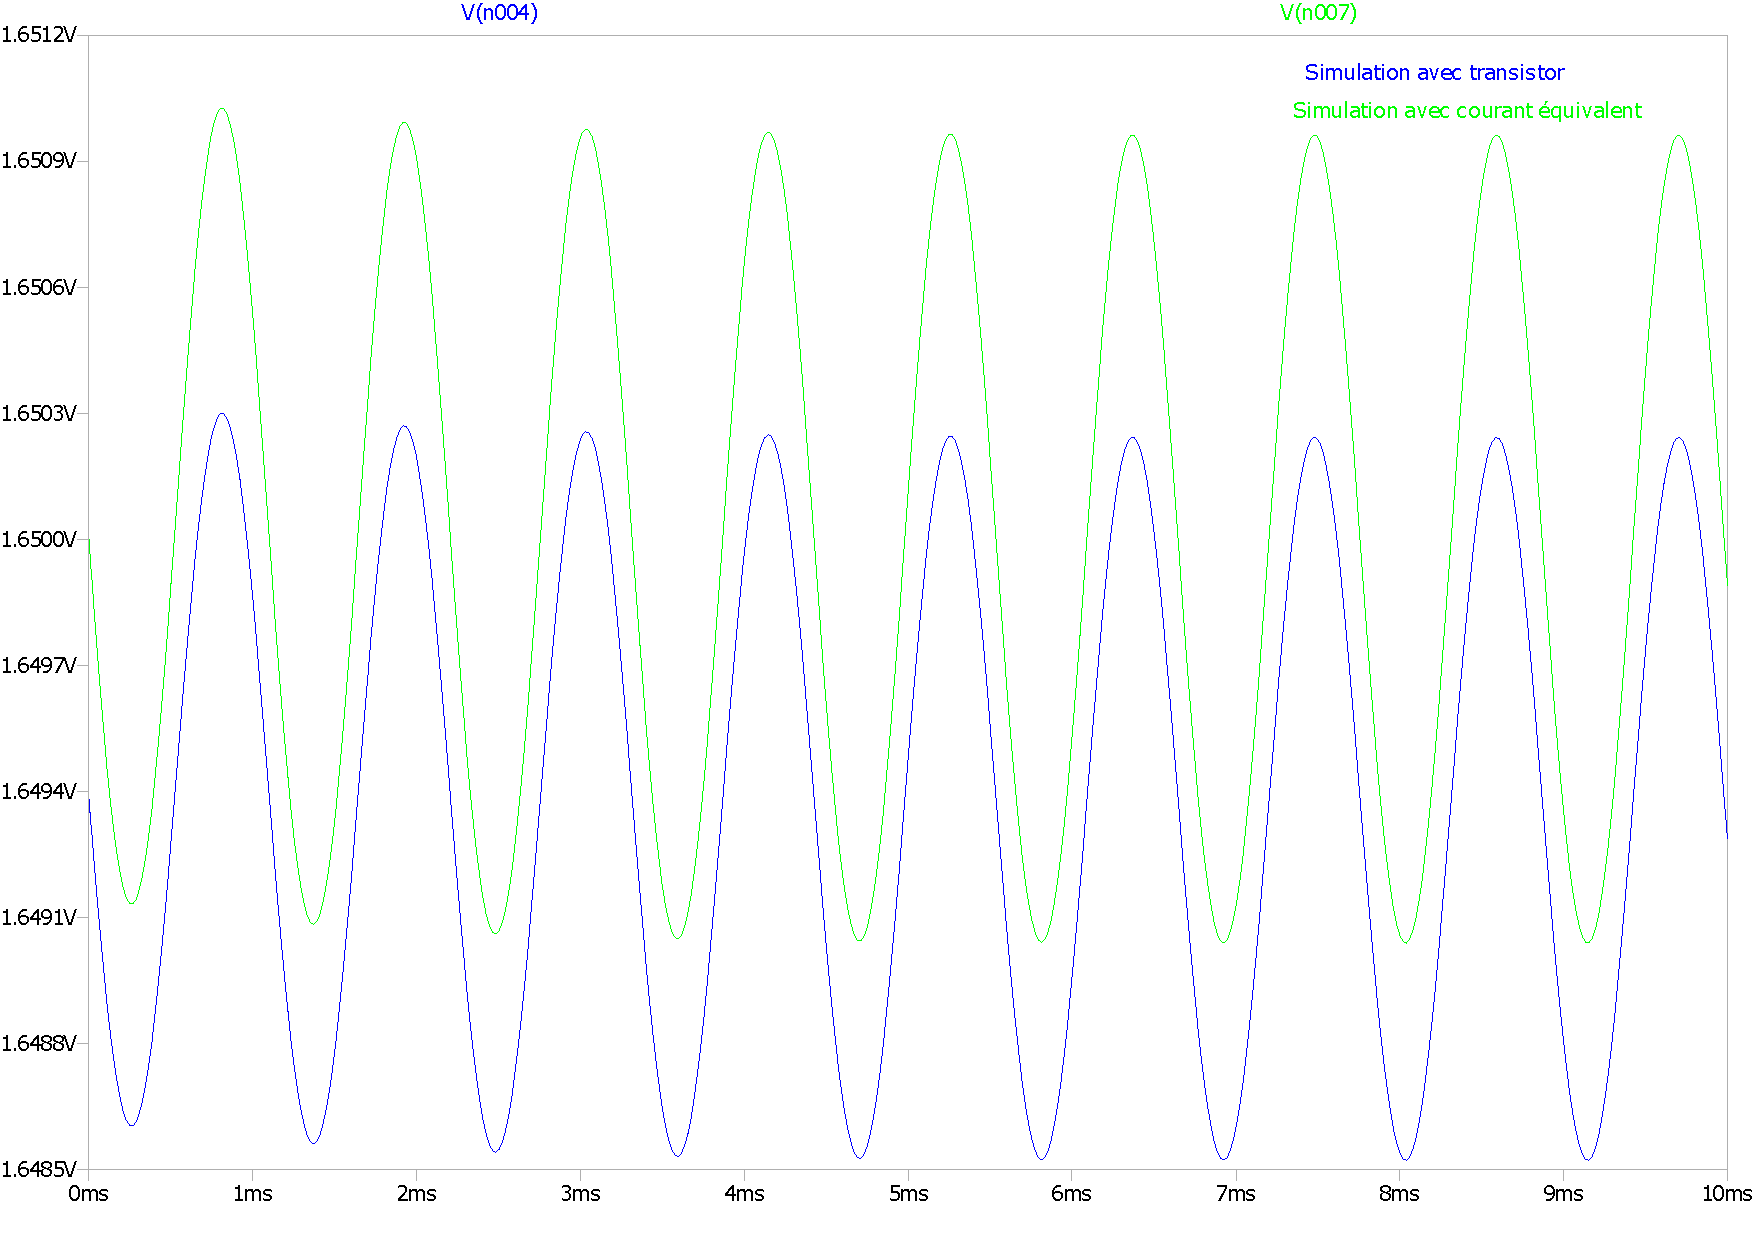
\includegraphics[width=0.7\textwidth]{pdffiles/HighPass/TransientJetVsCurrent.pdf}
%    \caption{Comparaison entre la réponse transitoire du circuit sur la figure \ref{fig:ltspice_current} et celui de la figure \ref{fig:ltspice_transistor}}
%    \label{fig:ltspiceHighPassResistors}
%\end{figure}

\section{Filtre de garde}\label{Lowpassfilterannexe}
\begin{figure}[H]
    \centering
    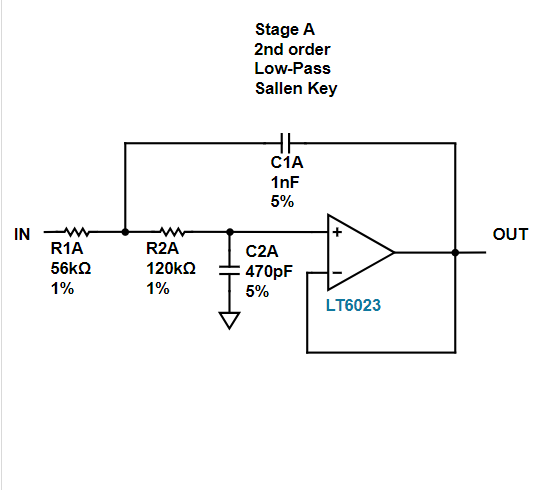
\includegraphics{Pictures/lowpass2.png}
    \caption{Filtre de garde}
    \label{fig:lowpassfilterannexe}
\end{figure}
\newpage
\begin{figure}[H]
    \centering
    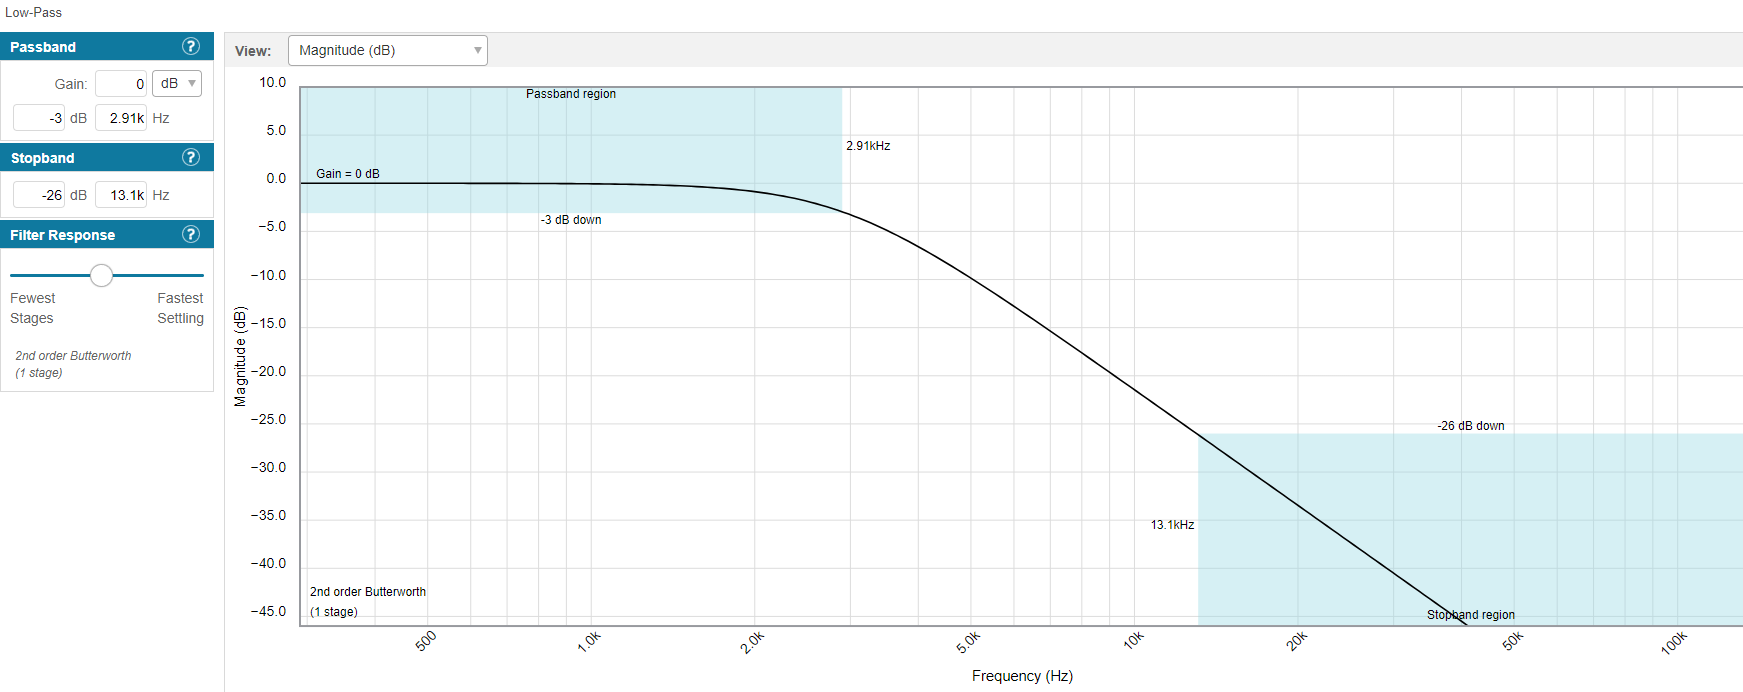
\includegraphics[width=1.5\textwidth,angle=90,origin=c]{Pictures/lowpassspecs.png}
    \caption{Gain du filtre de garde en dB}
    \label{fig:lowpassfiltermagnannexe}
\end{figure}

\section{Circuit de la chaîne d'acquisition}\label{chaineacquiannexe}
\begin{figure}[H]
    \centering
    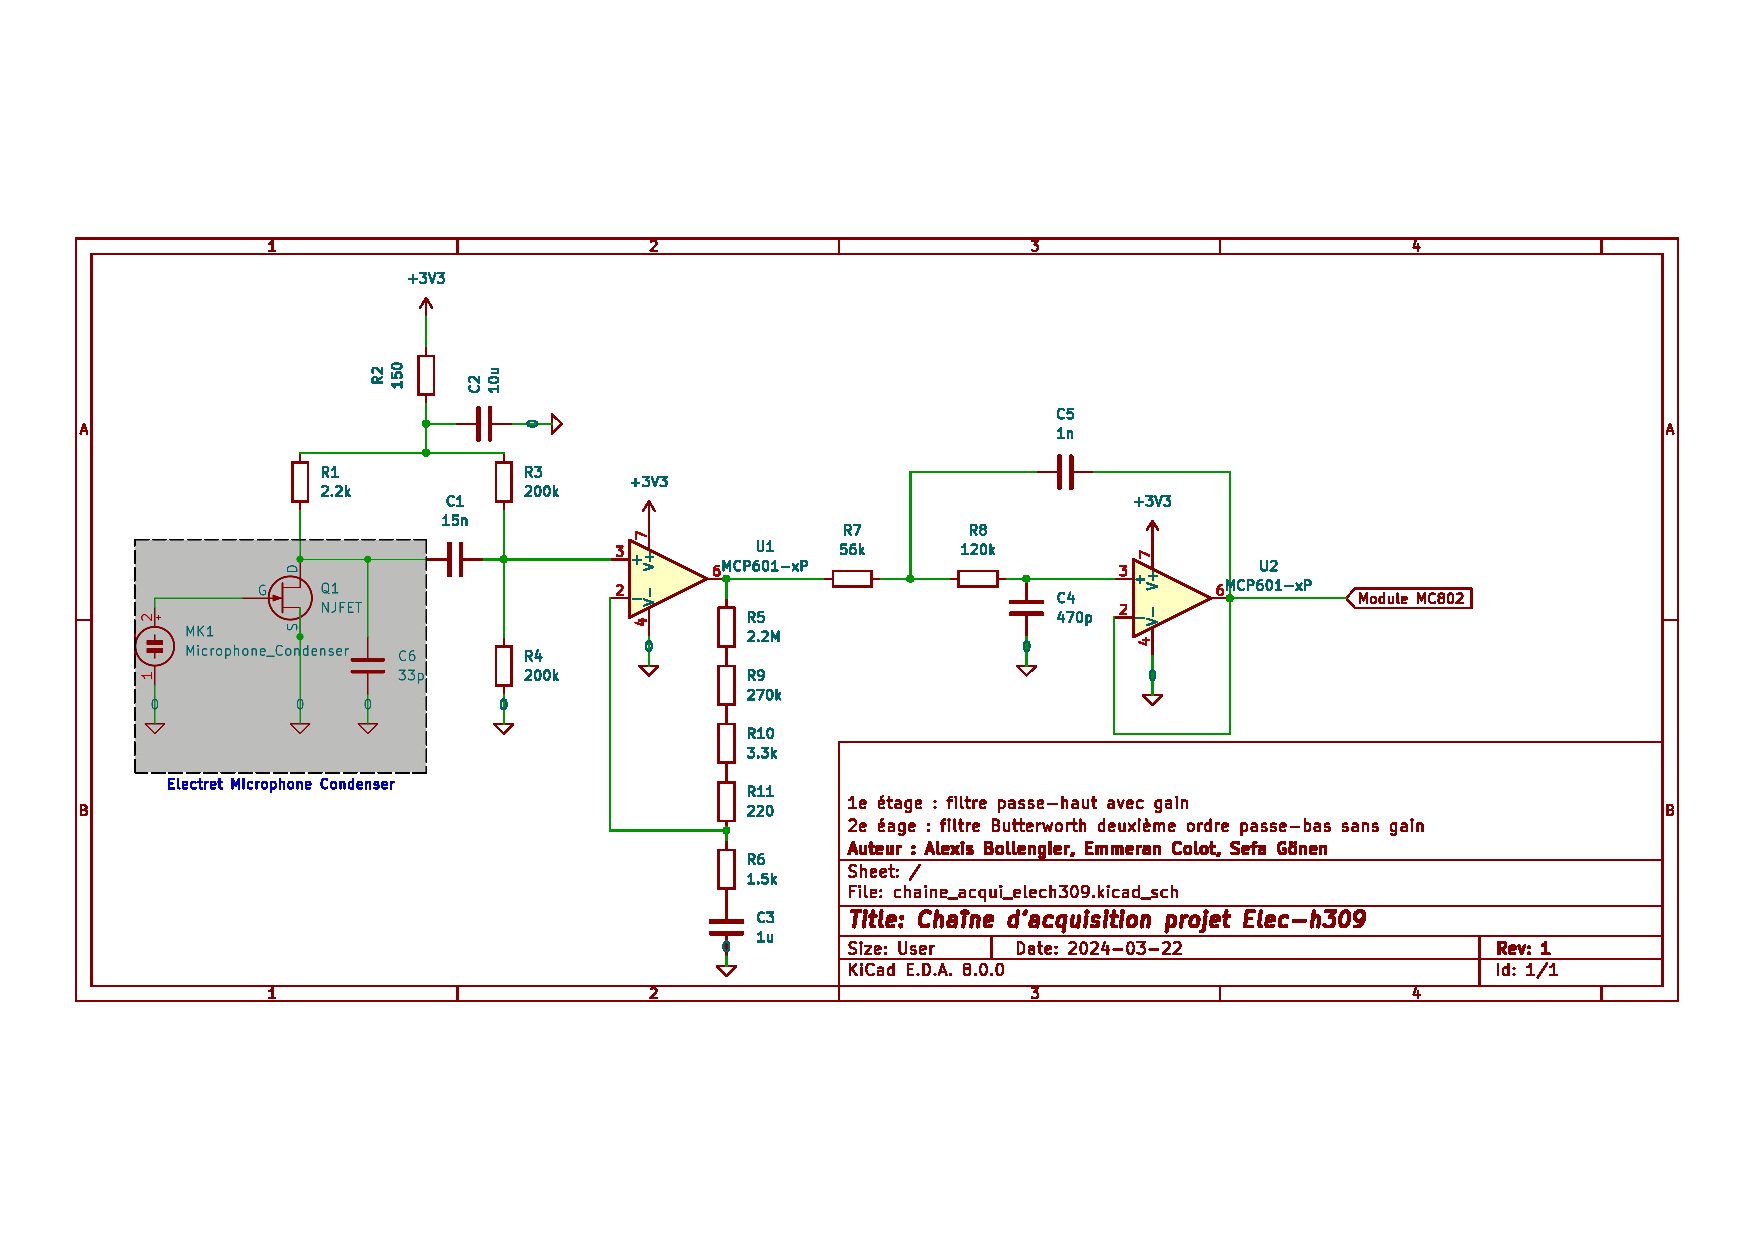
\includegraphics[width=1.4\textwidth,angle=90,origin=c]{pdffiles/chainacquiFullColor.pdf}
    \caption{Circuit de la chaîne d'acquisition}
    \label{fig:chainacquiannexe}
\end{figure}

%\section{Courbes de Bode de la chaîne d'acquisition}\label{Bodechaineacquiannexe}

%\begin{figure}[H]
%    \centering
%    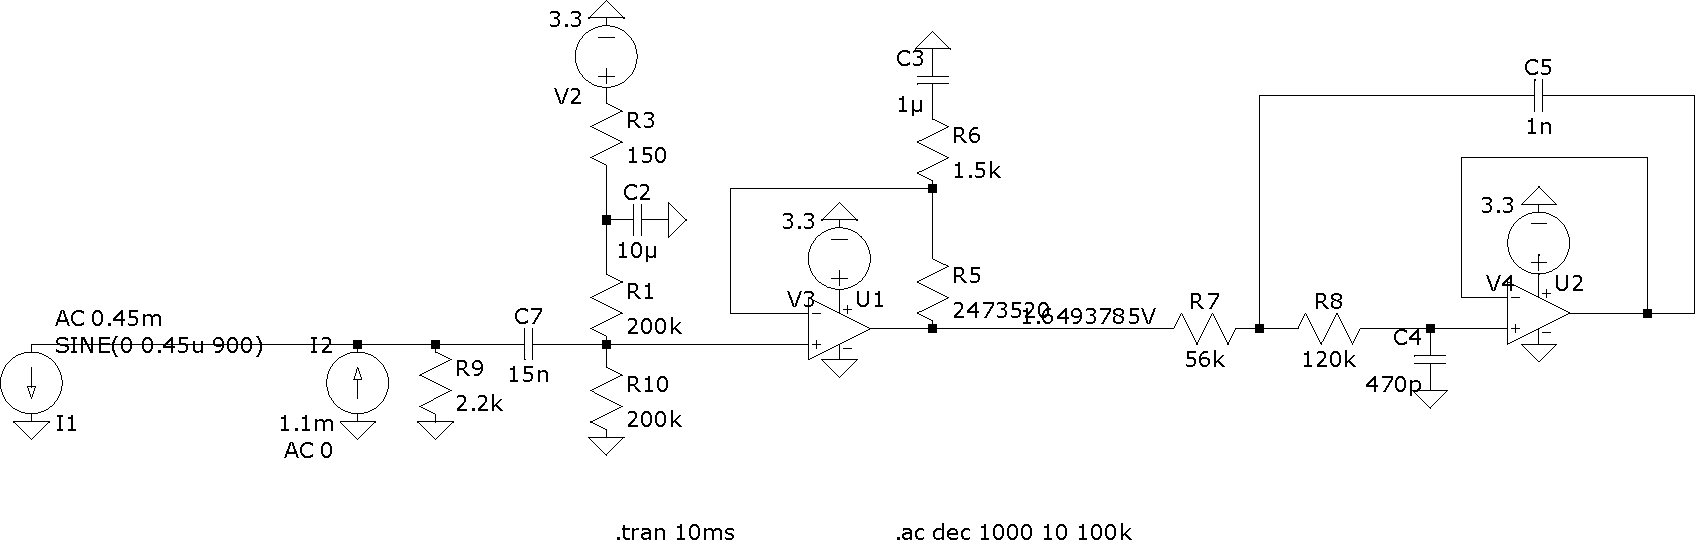
\includegraphics[width=\textwidth]{pdffiles/CircuitCurrent.pdf}
%    \caption{Circuit de simulation LTspice de la chaîne d'acquisition. Le microphone est remplacé par son équivalent source de courant}
%    \label{fig:circuitcurrentannexe}
%\end{figure}
%
%\begin{figure}[H]
%    \centering
%    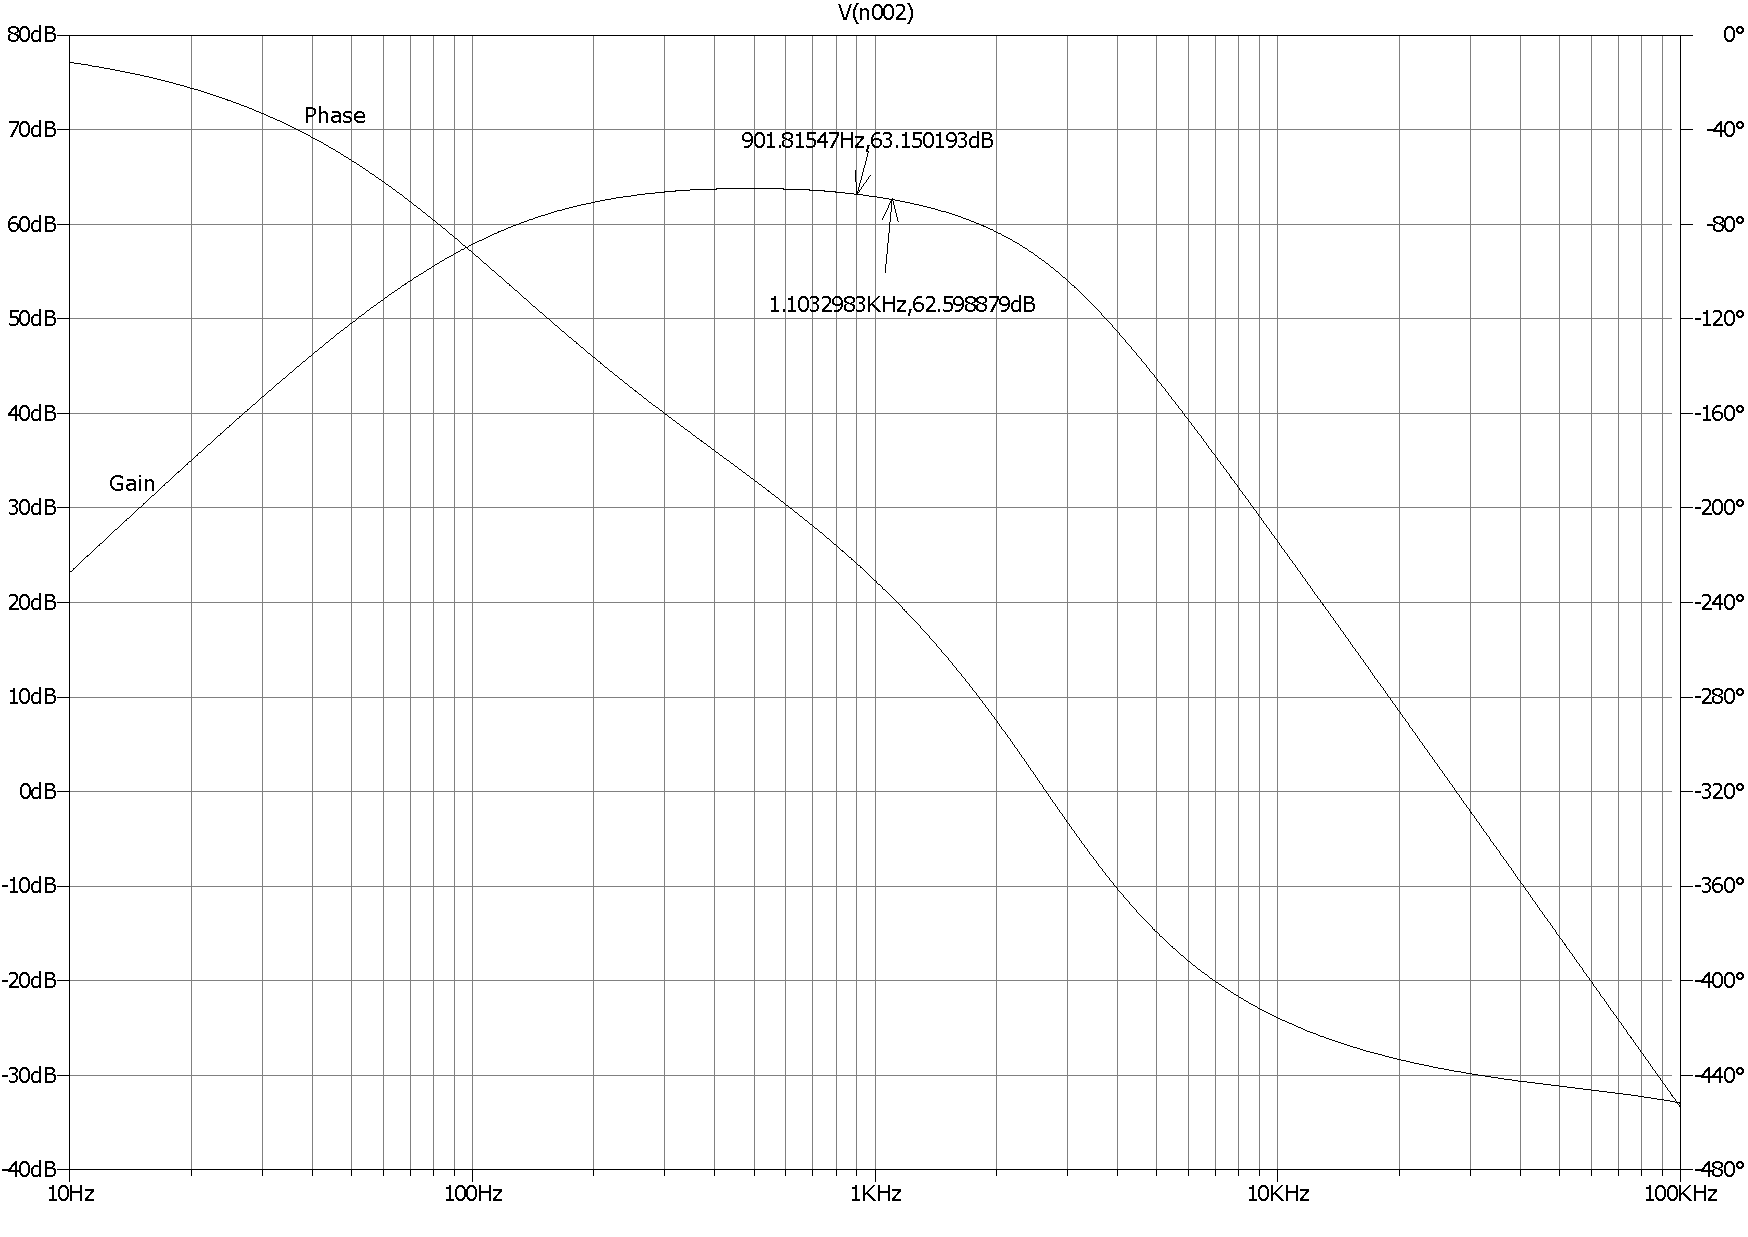
\includegraphics[width=\textwidth]{pdffiles/BodeCircuitCurrent.pdf}
%    \caption{Courbe de Bode de la chaîne d'acquisition. Le microphone est remplacé par son équivalent source de courant}
%    \label{fig:Bodecircuitcurrentannexe}
%\end{figure}
%
%\begin{figure}[H]
%    \centering
%    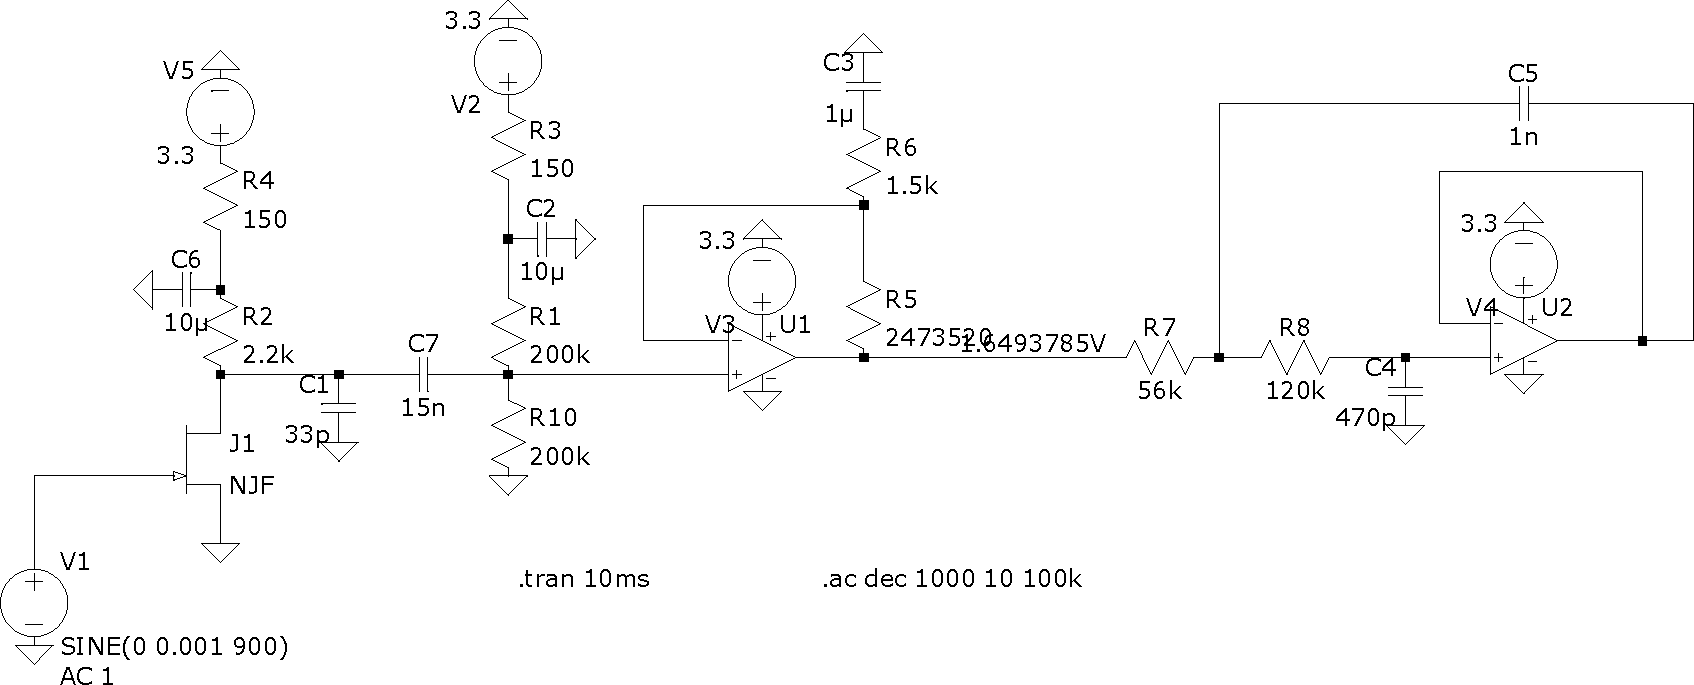
\includegraphics[width=\textwidth]{pdffiles/CircuitJET.pdf}
%    \caption{Circuit de simulation LTspice de la chaîne d'acquisition. Le microphone est remplacé par son équivalent transistor}
%    \label{fig:circuitjetannexe}
%\end{figure}
%
%\begin{figure}[H]
%    \centering
%    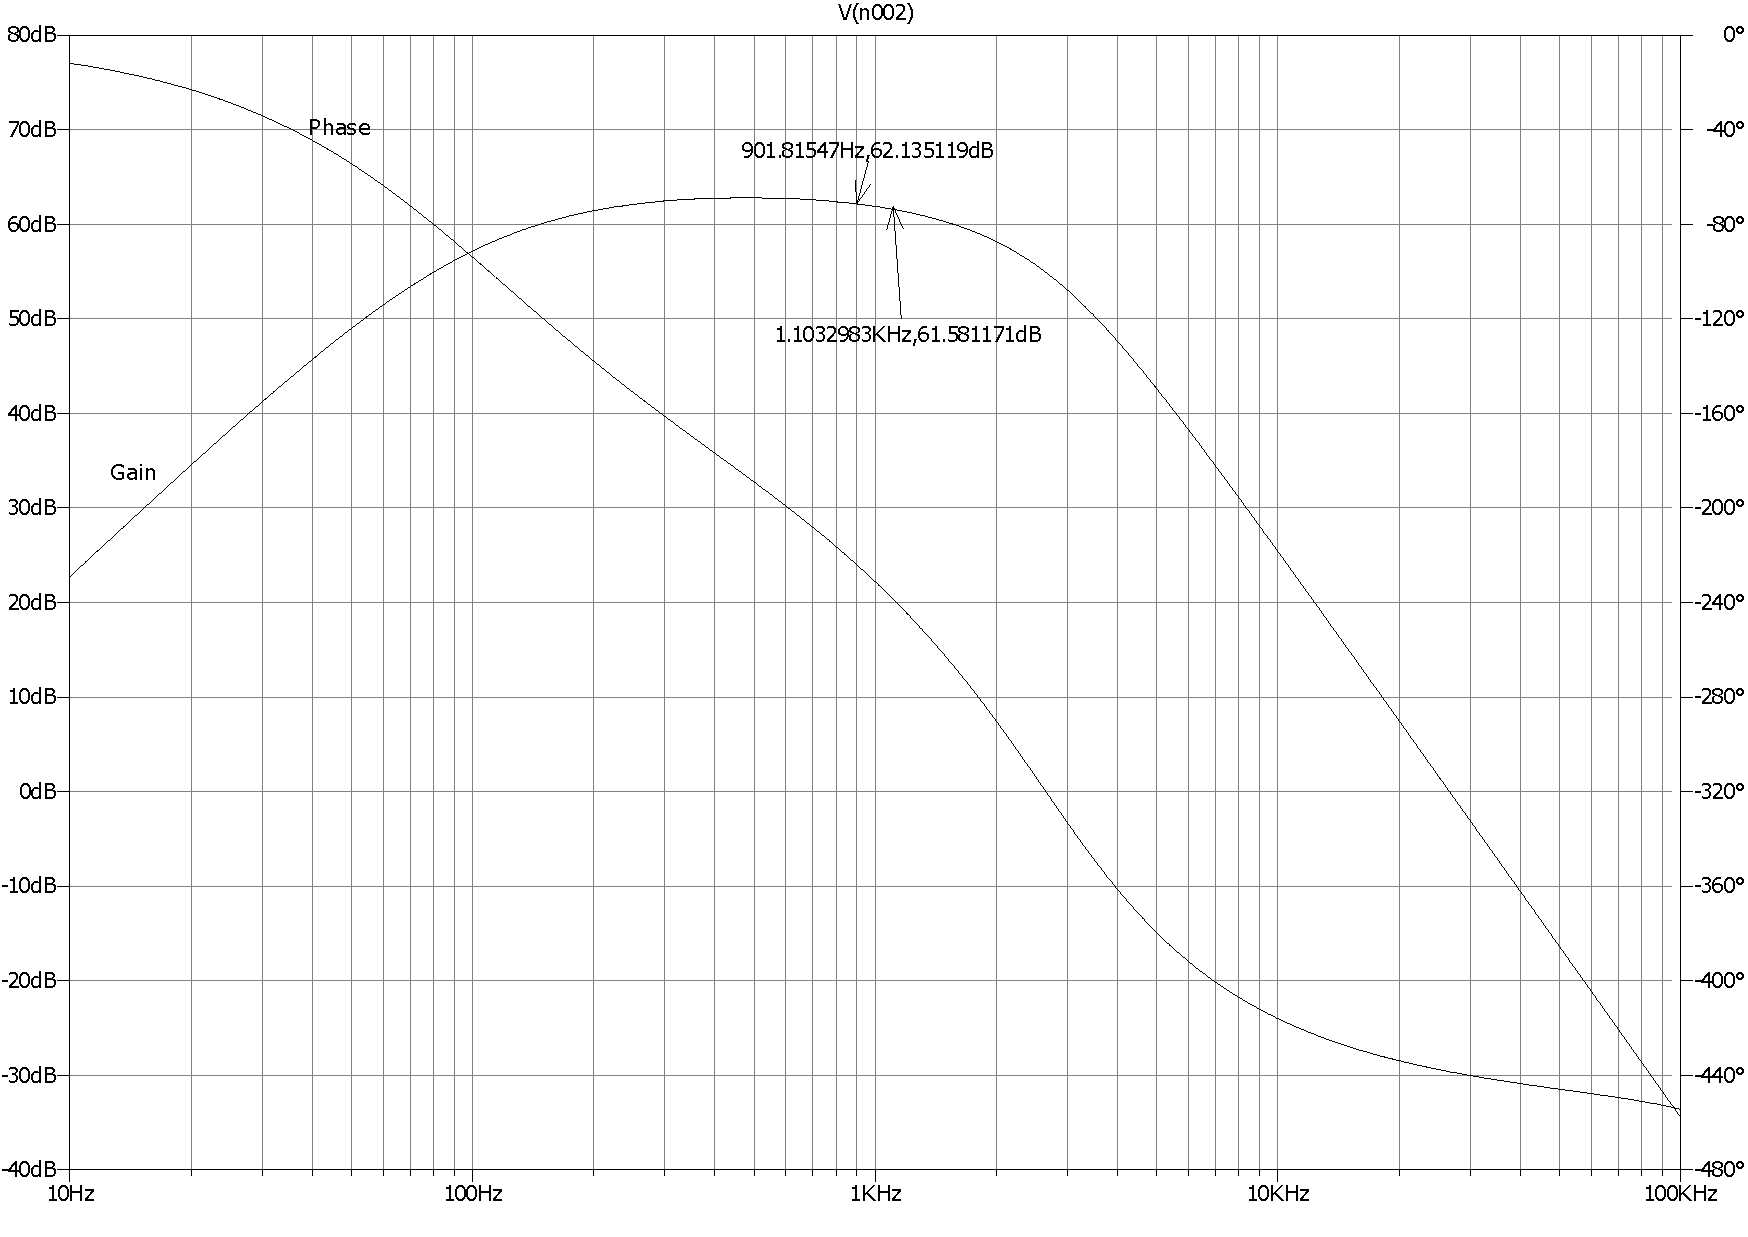
\includegraphics[width=\textwidth]{pdffiles/BodeCircuitJET.pdf}
%    \caption{Courbe de Bode de la chaîne d'acquisition. Le microphone est remplacé par son équivalent transistor}
%    \label{fig:Bodecircuitjetannexe}
%\end{figure}